% !TEX root = stack-thresh.tex

\section{Definitions and previous results}
\label{sec:previous}

In this section we present the problem setting and review previous results for Stackelberg routing on parallel networks with horizontal queues~\cite{krichene12}.




%-----------------------------------------------------------------------------------------------------------------------------------------------------------------
\subsection{Routing game on a parallel link with horizontal queues}
\label{sec:previous-Nash}

We consider a non-atomic routing game on a network of~$\NLinks$ parallel links, subject to flow demand~$\demand$ (see Figure~\ref{fig:network}). Each non-atomic player chooses a link ${n \in \{1, \dots, N\} }$ that minimizes their individual travel time, or latency, given by a function $\latency_n(\flow_n, \mode_n)$ of the total flow $\flow_n \in [0, \flowMax_n]$ and the congestion state $\mode_n \in \{0,1\}$ on the link. Here the latency on a link $n$ depends not only on the flow $\flow_n$, but on the congestion state of the link as well. By definition, the congestion state specifies whether the link is in free-flow $(\mode_n = 0)$ or is congested $(\mode_n = 1)$.
%
\begin{figure}[h]
\centering
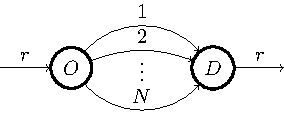
\includegraphics{TikZ/parallel_network.pdf}
\caption{Parallel network with $\NLinks$ links and demand~$\demand$.}
\label{fig:network}
\end{figure}
%
The latency functions are assumed to be in the HQSF class (horizontal queues, single-valued in free-flow) \cite{krichene12}, i.e. satisfies the following assumptions:
\begin{enumerate}
\item The latency in free-flow ${ \latency_n(\cdot, 0): [0, \flowMax_n] \rightarrow \Rbb_+ }$ is single-valued. We will denote by $a_n$ its value, called the \emph{free-flow latency}.
\item The latency in congestion $ \latency_n(\cdot, 1) : (0, \flowMax_n) \rightarrow (a_n, +\infty) $ is continuous decreasing.
\item Continuity: ${\lim_{\flow_n \rightarrow \flowMax_n} \latency(\flow_n, 1) = \latency_n(\flowMax_n, 0) = a_n}$
\end{enumerate}
We also assume that the free-flow latencies are distinct, and that the links are ordered by increasing free-flow latency, i.e.
\begin{equation}
\label{eq:index}
a_1 < a_2 < \dots < a_\NLinks
\end{equation}

Let $(\NLinks, \demand)$ denote an instance of the routing game, $\flowV \in \mathbb{R}_+^\NLinks$ the vector of flows, $\flowV^{\max} \in \Rbb_+^\NLinks$ the vector of capacities, and $\modeV \in \{0,1\}^\NLinks$ the vector of congestion states on the network. The assignment $(\flowV, \modeV)$ is said to be a feasible assignment if for every link $n$, the flow $\flow_n$ is admissible ($\flow_n \leq \flowMax_n$) and the total flow is conserved, i.e. $\sum_{n=1}^{\NLinks} \flow_n = \demand$. For a feasible assignment $(\flowV, \modeV)$, we define the total cost $C(\flowV, \modeV)$ as the sum of the latencies experienced by all users on all links
\[
C(\flowV, \modeV) = \sum_{n=1}^\NLinks {\latency_n(\flow_n, \mode_n) \flow_n}
\]

Let $\Supp{\flowV} = \{ n \in \{1, \dots, \NLinks\} | \flow_n > 0\}$ denote the support of a flow vector~$\flowV$.
\begin{definition}\emph{Nash equilibrium}\\
\label{def:NashEq}
A feasible assignment $(\flowV, \modeV)$ for the instance $(\NLinks, \demand)$ is a Nash equilibrium if there exists a positive latency $\latency_0 > 0$ such that
\begin{equation}
\begin{aligned}
n \in \Supp{\flowV} \Rightarrow \latency_n(\flow_n, \mode_n) = \latency_0 \\
n \notin \Supp{\flowV} \Rightarrow \latency_n(\flow_n, \mode_n) \geq \latency_0
\end{aligned}
\end{equation}
This means in particular that every user is experiencing the same travel time $\latency_0$. In this case the total cost of the equilibrium is simply~$C(\flowV, \modeV) = \demand \latency_0$. We will denote by $\std\NE$ the set of Nash equilibria of the instance $(\NLinks, \demand)$.
\end{definition}

\begin{definition}{\emph{Single-link free-flow equilibria and congestion flows}\\}
\label{def:CongFlow}
Let $(\flowV, \modeV) \in \std\NE$ be a Nash equilibrium, and let $k = \max \Supp{\flowV}$ be the last link (i.e. the one with the largest free-flow latency) in the support of~$\flowV$. If link $k$ is in free-flow, then $(\flowV, \modeV)$ is said to be a single-link-free-flow equilibrium, and satisfies the following properties:
\begin{itemize}
\item $\Supp{\flowV} = \{1, \dots, k\}$
\item The common latency on the support of~$\flowV$ is $a_k$
\item The flow on links $n \in \{1, \dots, k-1\}$ is given by the congestion flows $\cFlow{n}{k}$ defined by
\[
\cFlow{n}{k} = \latency_n(.,1)^{-1}(a_k)
\]
\end{itemize}
Therefore a single-link-free-flow equilibrium is of the form
\begin{align*}
\modeV &= (1, \dots, 1, \overbracBig{0}{k}, \dots, 0) \\
\flowV &= \big( \cFlow{1}{k}, \dots, \cFlow{k-1}{k}, \overbracBig{\demand - \sum_{n=1}^{k-1}\cFlow{n}{k}}{k}, 0, \dots, 0 \big)
\end{align*}
\end{definition}

Figure~\ref{fig:ff_nash} shows an example of a single-link-free-flow equilibrium on an instance with $\NLinks = 4$ links. We observe that the congestion flow $\cFlow{n}{k}$ is a decreasing function of $k$ since $k \mapsto a_k$ is increasing by assumption~\eqref{eq:index} and $\latency_n(\cdot, 1)$ is decreasing.
%%%
\begin{figure}[h]
\centering
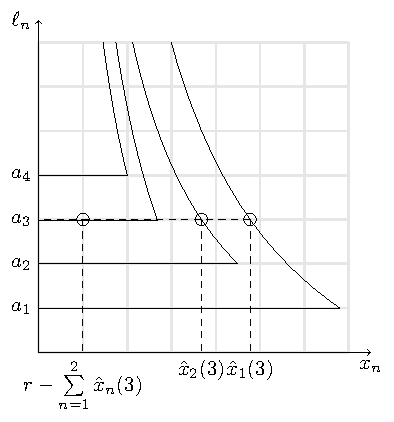
\includegraphics[width=2.5in]{TikZ/ff_nash.pdf}
\caption{Example of a single-link-free-flow equilibrium.}
\label{fig:ff_nash}
\end{figure}
%

\begin{definition}
\label{def:maxDemand}
We denote, for any $k\in \{1,\ldots,N\}$, by $\demandMax{k}$ the maximum demand such that the set of Nash equilibria $\NE{k}{\demand}$ is non-empty. It is given by
\begin{equation}
\demandMax{k} = \max_{ j \in \{1,\dots, k\} } \{\flowMax_j + \sum_{n=1}^{j-1} \cFlow{n}{j} \}
\end{equation}
\end{definition}

\begin{remark}
\label{remark:maxDemand}
We also have the following property: a single-link-free-flow equilibrium exists for the instance $(k, \demand)$ if and only if $\demand \leq \demandMax{k}$.
\end{remark}

Proofs of these facts are given in Lemma~1 and Corollary~2 in~\cite{krichene12}, and they are provided in the Appendix for completeness. By definition, we have $\forall k \in \{2, \dots, \NLinks \}$, ${ \demandMax{k} \geq \demandMax{k-1} }$. We will be interested, in particular, in links that strictly increase the maximum demand, i.e. such that $\demandMax{k} > \demandMax{k-1}$. We denote these links by $k_1, \dots, k_c$, defined by induction as follows:
\begin{align}
& k_1 = 1 \\
& \forall i \in \{2, \dots, c\}, \ k_{i} = \min \{n \leq \NLinks | \demandMax{n} > \demandMax{k_{i-1}}\} \label{eq:nj}
\end{align}
Therefore we have
\[
\demandMax{1} = \demandMax{k_1} < \dots < \demandMax{k_c} = \demandMax{\NLinks}
\]
Here $c$ is the number of distinct elements in the set $\{\demandMax{k}, k \in \{1, \dots, \NLinks\}\}$.


\begin{definition}{\emph{Best Nash equilibrium}\\}
\label{def:BstNashEq}
The set of best Nash equilibria is the set of Nash equilibria that minimize the system-wide latency. 
\begin{equation}
\std \BNE = \underset{(\flowV, \modeV) \in \std\NE}{\arg\min} C(\flowV, \modeV)
\end{equation}
\end{definition}

\begin{remark}
\label{remark:smallest-support}
It is shown in~\cite{krichene12} (Lemma~3) that the best Nash equilibrium is unique, and that it is equal to the single-link-free-flow equilibrium with smallest support. With a slight abuse of notation, we will use $\std \BNE$ to denote the unique best Nash equilibrium (identifying the set with its unique element).
\end{remark}

\begin{proposition}\emph{Last link in the support of a best Nash equilibrium}\\
\label{prop:lastNash}
Let $(\flowV, \modeV)$ be the best Nash equilibrium for the instance $(\NLinks, \demand)$, then the last link in the support of~$\flowV$ is given by
\begin{equation}
\max \Supp{\flowV} = \min \left\{k: r \leq \demandMax{k} \right\}
\end{equation}
\end{proposition}

\begin{proof}
Let $b = \max \Supp{\flowV}$. Since an equilibrium exists for the instance~$(b, \demand)$, then $\demand \leq \demandMax{b}$ by Definition~\ref{def:maxDemand} of the maximum demand. And for all $k$ such that $\demand \leq \demandMax{k}$, by Remark~\ref{remark:maxDemand}, there exists a single-link-free-flow equilibrium supported on  $\{1, \dots, k\}$, thus by Remark~\ref{remark:smallest-support}, $k \geq b$. Therefore $b$ is the minimum such index.
\end{proof}

%-----------------------------------------------------------------------------------------------------------------------------------------------------------------
\subsection{Stackelberg routing game}
\label{sec:previous-Stack}

In the Stackelberg routing game, a central coordinator controls a fixed fraction of the total flow. This~\emph{compliant flow} corresponds to players who are either altruistic and care about the system-wide latency, or who may have an external incentive to be controlled by the coordinator. First, the coordinator (the leader) chooses the routes of the compliant flow. The resulting vector of flows is called a Stackelberg strategy and denoted by $\sV$. It satisfies $\sum_{n = 1}^\NLinks s_n = \compRate \demand$. Then the strategy $\sV$ of the leader is revealed, and the remaining players (the followers, corresponding to non-compliant flow $(1-\compRate) \demand$) choose their routes selfishly. The resulting non-compliant assignment, \emph{induced} by Stackelberg strategy~$\sV$, is denoted by $(\tV(\sV), \modeV(\sV))$. It is assumed to be the best Nash equilibrium \cite{krichene12} and satisfies the following: there exists a common latency $\latency_0$ on the support of $\tV(\sV)$ such that
\begin{equation}
\label{eq:induced_eq}
\begin{aligned}
n \in \Supp{\tV(\sV)} &\Rightarrow \latency_n(t_n(\sV) + s_n, \mode_n(\sV)) = \latency_0 \\
n \notin \Supp{\tV(\sV)} &\Rightarrow \latency_n(s_n, \mode_n(\sV)) \geq \latency_0
\end{aligned}
\end{equation}

We will denote by $(\NLinks, \demand, \compRate)$ an instance of the Stackelberg game played on a network with $\NLinks$ parallel links, demand~$\demand$ and compliance rate~$\compRate$. The leader seeks to minimize the system-wide latency, or total cost, induced by the Stackelberg strategy~$\sV$, and given by~$C(\sV + \tV(\sV), \modeV(\sV))$. The total assignment $(\sV + \tV(\sV), \modeV(\sV))$ is called the Stackelberg equilibrium induced by $\sV$.

\begin{definition}{\emph{Optimal Stackelberg strategies}\\}
\label{def:BstStck}
The set of optimal Stackelberg strategies $S^\star(\NLinks, \demand, \compRate)$ is the set of Stackelberg strategies that minimize the system-wide latency of the total flow induced by~$\sV$
\begin{equation}
\stdStack \stackSetOpt = \underset{\sV \in \stdStack\stackSet}{\arg\min} C(\sV+\tV(\sV), \modeV(\sV))
\end{equation}
\end{definition}

We will focus on one particular optimal Stackelberg strategy, the non-compliant first strategy (NCF). It is defined as follows:
\begin{definition}\emph{The non-compliant first strategy}
\\
Consider the Stackelberg instance $(\NLinks, \demand, \compRate)$. Let ${ (\tV^{(\cR)}, \modeV^{(\cR)}) = \BNE{\NLinks}{(1 - \compRate) \demand} }$ be the unique best Nash equilibrium of the non-compliant flow~$(1-\compRate) \demand$, and $\lastNC{\cR} = \max \supp(\tV^{(\cR)})$ be the last link in its support. Then the non-compliant first strategy is the Stackelberg strategy given by
\begin{multline}
\stdStack\NCF = \bigg( 0, \dots, \overbracBig{0}{\lastNC{\cR}-1}, \overbracBig{\flowMax_{\lastNC{\cR}}-t^{(\cR)}_{\lastNC{\cR}}}{\lastNC{\cR}}, \flowMax_{\lastNC{\cR}+1}, \dots, \\
\flowMax_{\lastStack{\cR}-1}, \compRate\demand - \bigg( \sum_{n = \lastNC{\cR}}^{\lastStack{\cR}-1} \flowMax_n-t^{(\cR)}_{\lastNC{\cR}} \bigg), 0, \dots, 0 \bigg)
\label{eq:NCF}
\end{multline}

where $\lastStack{\cR}$ is the maximal index $l \in \{\lastNC{\cR}+1 , \dots, \NLinks \}$ such that ${\alpha r - \big( \sum_{n = \lastNC{\cR}}^{l-1} \flowMax_n - t^{(\cR)}_{\lastNC{\cR}} \big) > 0} $. By definition, $\lastStack{\cR}$ is the last link in the support of $\stdStack \NCF$. We will also use $\sV^{(\cR)}$ as a shorthand for $\stdStack \NCF$\footnote{Since we will consider instances with fixed demand and fixed number of links, we use superscript $\compRate$ to emphasize the dependency on the compliance rate.}.
\end{definition}

\begin{figure}[h]
\centering
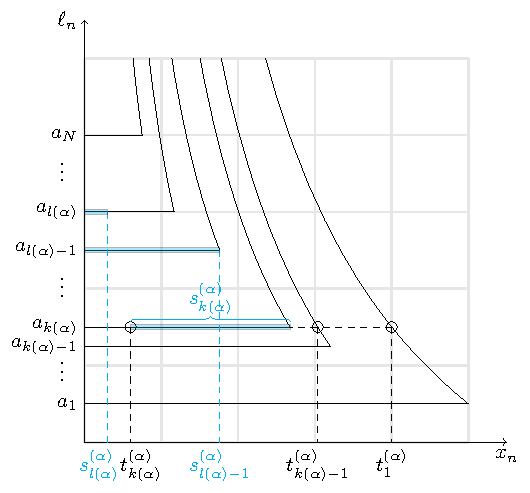
\includegraphics[width=3.3in]{TikZ/stack_NCF_new.pdf}
\caption{Illustration of the NCF strategy. The best Nash equilibrium of the non-compliant flow is given by $(\tV^{(\cR)}, \modeV^{(\cR)})$ (circles) and the NCF strategy~$\sV^{(\cR)}$ is highlighted in blue.}
\label{fig:ncf}
\end{figure}

The NCF strategy saturates links one by one starting from~$\lastNC{\cR}$, the last link in the support of $\tV^{(\cR)}$, until the compliant flow $\alpha \demand$ is completely assigned. Fig.~\ref{fig:ncf} gives an illustration of the NCF strategy. The Non-compliant-first strategy is shown to be an optimal Stackelberg strategy in~\cite{krichene12}.

We note that the induced non-compliant equilibrium $( \tV^{(\cR)}, \modeV^{(\cR)} )$ is given by
\begin{align}
\modeV^{(\cR)} &= \big( 1, \dots, 1, \overbracBig{0}{\lastNC{\cR}}, \dots, 0 \big) \label{eq:NCF-ncMode}\\
\tV^{(\cR)} &= \big( \cFlow{1}{\lastNC{\cR}}, \dots, \cFlow{\lastNC{\cR} - 1}{\lastNC{\cR}}, t^{(\cR)}_{\lastNC{\cR}}, 0, \dots, 0 \big) \label{eq:NCF-ncFlow}
\end{align}
the total flow $\flowV^{(\cR)} = \sV^{(\cR)} + \tV^{(\cR)}$ is given by
\begin{multline}
\flowV^{(\cR)} = \big( \cFlow{1}{\lastNC{\cR}}, \dots, \cFlow{\lastNC{\cR} - 1}{\lastNC{\cR}}, \\
\flowMax_{\lastNC{\cR}}, \dots, \flowMax_{\lastStack{\cR} - 1}, 
\flow_{\lastStack{\cR}}, 0, \dots, 0 \big)
\label{eq:NCF-totalFlow}
\end{multline}
where $\flow_{\lastStack{\cR}}$ is simply given by
\[
\flow_{\lastStack{\cR}} = \demand - \sum_{n = 1}^{\lastNC{\cR} - 1} \cFlow{n}{\lastNC{\cR}} - \sum_{n = \lastNC{\cR}}^{\lastStack{\cR} - 1} \flowMax_n
\]
Finally, the latencies are given by
\[
(a_{\lastNC{\cR}}, \dots, \overbracBig{a_{\lastNC{\cR}}}{\lastNC{\cR}}, a_{\lastNC{\cR}+1}, \dots, a_{\NLinks} )
\]
All these results are summarized in Fig.~\ref{fig:ncf}